\documentclass[aspectratio=169]{beamer}


\mode<presentation>
{
  \usetheme{Antibes}

  \setbeamercovered{transparent}
}

% Remove the subsection bar.
\makeatletter
\setbeamertemplate{headline}
{%
    \begin{beamercolorbox}[wd=\paperwidth,colsep=1.5pt]{upper separation line head}
    \end{beamercolorbox}
    \begin{beamercolorbox}[wd=\paperwidth,ht=2.5ex,dp=1.125ex,%
      leftskip=.3cm,rightskip=.3cm plus1fil]{title in head/foot}
      \usebeamerfont{title in head/foot}\insertshorttitle
    \end{beamercolorbox}
    \begin{beamercolorbox}[wd=\paperwidth,ht=2.5ex,dp=1.125ex,%
      leftskip=.3cm,rightskip=.3cm plus1fil]{section in head/foot}
      \usebeamerfont{section in head/foot}%
      \ifbeamer@tree@showhooks
        \setbox\beamer@tempbox=\hbox{\insertsectionhead}%
        \ifdim\wd\beamer@tempbox>1pt%
          \hskip2pt\raise1.9pt\hbox{\vrule width0.4pt height1.875ex\vrule width 5pt height0.4pt}%
          \hskip1pt%
        \fi%
      \else%  
        \hskip6pt%
      \fi%
      \insertsectionhead
    \end{beamercolorbox}
% Code for subsections removed here
}
\makeatother


\usepackage[french]{babel}
\usepackage[utf8]{inputenc}
\usepackage{times}
\usepackage[T1]{fontenc}
\usepackage{xcolor}
\usepackage{booktabs}
\usepackage{threeparttable}
\usepackage{tabularx}
\usepackage{caption}
\usepackage{numprint}
\usepackage{amsmath,amsfonts,amsthm,bm,nccmath}
\usepackage[export]{adjustbox}
\usepackage{tikz}
\usepackage{float}
\usepackage{listings}
\usepackage{textcomp}
\usepackage[backend=biber, style=authoryear, defernumbers=true]{biblatex}

\addbibresource{MyLibrary.bib}

\renewcommand*{\bibfont}{\scriptsize}

\captionsetup{font=scriptsize, labelfont=scriptsize}

\date{8 décembre 2022}

%\usefonttheme[onlymath]{serif}

\definecolor{my_blue}{rgb}{0.3, 0.4, 0.5}
\definecolor{my_grey}{rgb}{0.6, 0.6, 0.6}
\definecolor{inrs_blue}{rgb}{0.0627451, 0.1176471, 0.2588235}

\usecolortheme[named = my_blue]{structure}

\setbeamertemplate{footline}{}

\setbeamerfont{author in head/foot}{size=\fontsize{4}{4.8}\selectfont}

\setbeamertemplate{bibliography item}{}
\setbeamertemplate{bibliography entry article}{}
\setbeamertemplate{bibliography entry title}{}
\setbeamertemplate{bibliography entry location}{}
\setbeamertemplate{bibliography entry note}{}


\setbeamerfont{bibliography entry author}{size=\footnotesize}
\setbeamerfont{bibliography entry title}{size=\footnotesize}
\setbeamerfont{bibliography entry location}{size=\footnotesize}
\setbeamerfont{bibliography entry note}{size=\footnotesize}

\defbeamertemplate{footline}{myframe number}
{
  \hfill%
  \usebeamercolor[fg]{page number in head/foot}%
  \usebeamerfont{page number in head/foot}%
  \raisebox{0.3cm}[0pt][0pt]{% <--- change here
    \insertframenumber\,/\,\inserttotalframenumber\kern1em}%
}

\setbeamertemplate{footline}[myframe number]
\beamertemplatenavigationsymbolsempty

\newcommand\Wider[2][3em]{%
\makebox[\linewidth][c]{%
  \begin{minipage}{\dimexpr\textwidth+#1\relax}
  \raggedright#2
  \end{minipage}%
  }%
}


\title{Modélisation nonstationnaires des valeurs extrêmes par reversible jump Markov chain Monte Carlo}

\author{Antoine~Chapon~et Jean Truchard Saint Clore}

\institute[Universities of Somewhere and Elsewhere] % (optional, but mostly needed)
{
  cours ETE 405
 }
% - Use the \inst command only if there are several affiliations.
% - Keep it simple, no one is interested in your street address.

%\date[CFP 2003] % (optional, should be abbreviation of conference name)
%{Conference on Fabulous Presentations, 2003}
% - Either use conference name or its abbreviation.
% - Not really informative to the audience, more for people (including
%   yourself) who are reading the slides online

%\subject{Theoretical Computer Science}
% This is only inserted into the PDF information catalog. Can be left
% out. 



% If you have a file called "university-logo-filename.xxx", where xxx
% is a graphic format that can be processed by latex or pdflatex,
% resp., then you can add a logo as follows:

%\pgfdeclareimage[height=2cm]{logoINRS}{Logo-INRS-horizontal.png}
%\logo{\pgfuseimage{logoINRS}}

\titlegraphic{\vspace{-0.5cm}\flushleft
\includegraphics[width=2.5cm]{Logo-INRS-horizontal.png}}

% Delete this, if you do not want the table of contents to pop up at
% the beginning of each subsection:
\AtBeginSection[] % \AtBeginSubsection[]
{
\begin{frame}<beamer>{Plan}
\frametitle{Plan}
\tableofcontents[currentsection,currentsubsection]
\end{frame}
}


% If you wish to uncover everything in a step-wise fashion, uncomment
% the following command: 

%\beamerdefaultoverlayspecification{<+->}


\begin{document}

\begin{frame}
  \titlepage
\end{frame}



\section*{}

\begin{frame}{Introduction}
Analyse fréquentielle des évènements extrêmes avec :
\vspace{0.5cm}
\begin{itemize}
\setlength{\itemsep}{10pt}
	\item modèle par dépassement de seuil,
	\item nonstationnarité,
	\item incertitudes.
\end{itemize}
\vspace{0.5cm}
Échantillonnage des paramètres du modèle et échantillonnage des différents modèles nonstationnaires avec une approche Bayesienne.
\end{frame}

\begin{frame}{Plan}
\tableofcontents
\end{frame}


\section{Modèle nonstationaire des valeurs extrêmes par dépassement de seuil}


\begin{frame}{Variable modélisée}
\begin{columns}
	\begin{column}{0.65\textwidth}
	\vspace{-1.2cm}
	\begin{figure}
	 		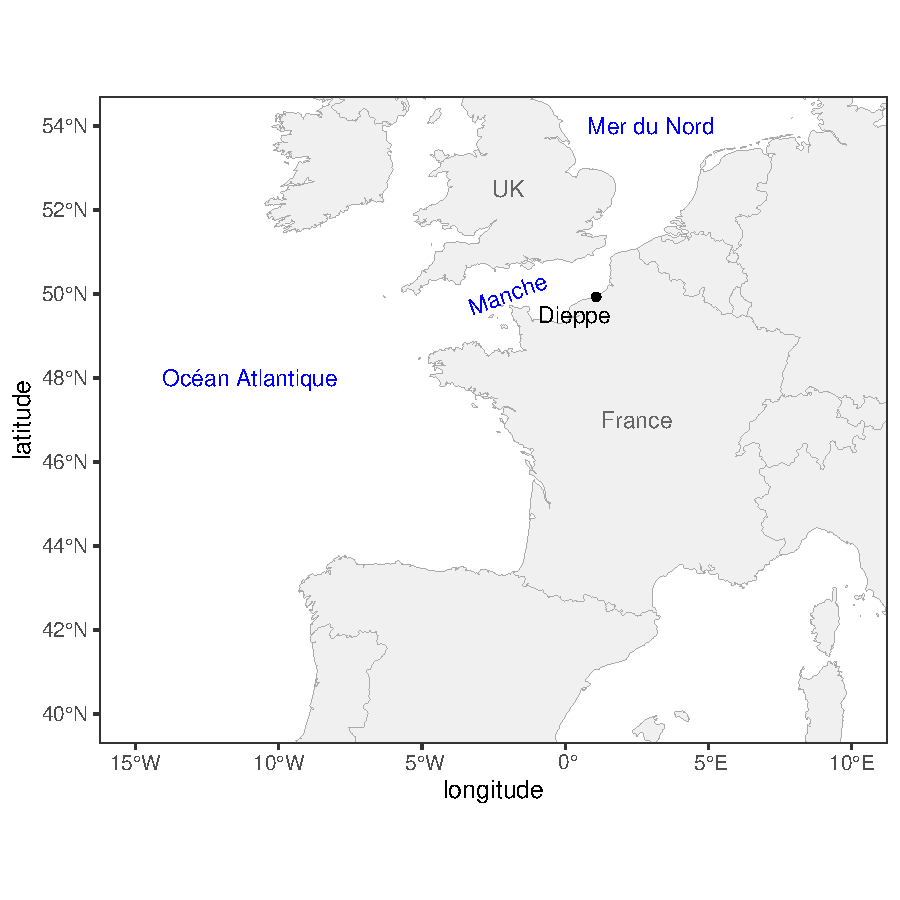
\includegraphics[height=1.1\textheight, center]{../figures/map.pdf}
	\end{figure}
	\end{column}
	\begin{column}{0.35\textwidth}
	\vspace{-1cm}\\
	\begin{itemize}
	\setlength{\itemsep}{17pt}
	\item Surcote marine (ici skew surge) journalière : différence entre le niveau marin observé et la marée prédite.
	\item Modification locale et transitoire du niveau marin causée par la dépression atmosphérique et le vent.
	\end{itemize}
	\end{column}
\end{columns}
\end{frame}


\begin{frame}{Approche Peaks Over Threshold}
\begin{itemize}
	\setlength{\itemsep}{17pt}
	\item Rééchantillonnage pour extraire les évènements extrêmes.
	\item Un évènement extrême peut correspondre à plusieurs dépassements consécutifs (fréquence d'observation journalière).
	\item Seule les valeurs maximale des clusters de dépassements sont gardées comme valeurs extrêmes.
	\item Run declustering : clusters distincts définis par $r$ valeurs sous le seuil.
	\item 46 ans de données.
\end{itemize}
\end{frame}


\begin{frame}{Seuil par régression quantile}
\begin{columns}
	\begin{column}{0.4\textwidth}
		\begin{figure}
		\vspace{-0.4cm}
	 		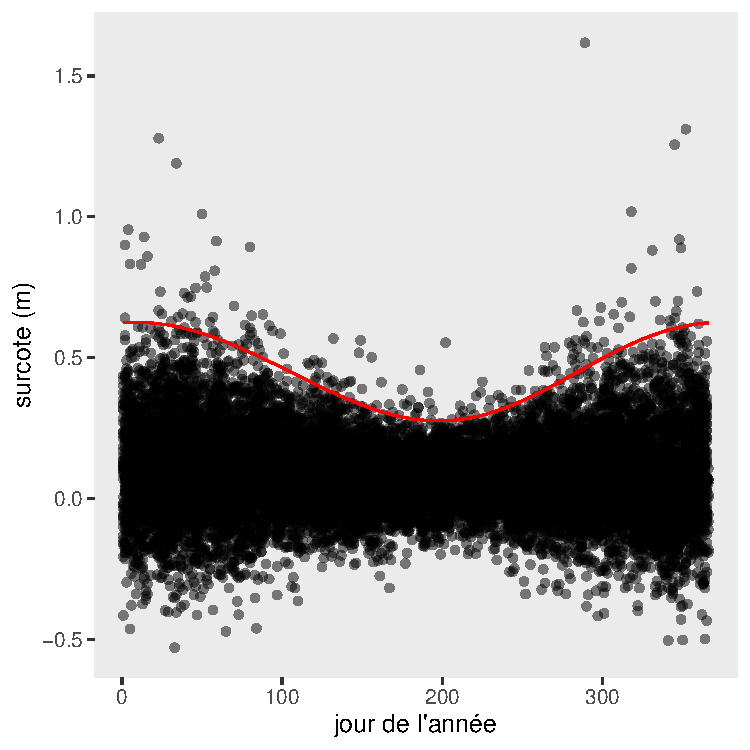
\includegraphics[height=0.875\textheight, center]{../figures/points.pdf}
		\end{figure}
	\end{column}
	\begin{column}{0.6\textwidth}
	\begin{itemize}
	\setlength{\itemsep}{10pt}
	\item Forte saisonnalité du signal.
	\item Régression quantile $\tau = 0.99$ (données journalières) en fonction de la saison modélisé par une sinusoïde.
	\item En minimisant
	\end{itemize}
	\begin{equation*}
	\ell_u = \tau \sum_{i|r_i \geq 0} |r_i| + (1-\tau) \sum_{i|r_i < 0} |r_i|
	\end{equation*}
	\phantom{-----.} avec $r_i$ le rang de l'observation $i$. %no one will ever know
	\end{column}
\end{columns}
\end{frame}


\begin{frame}{Nonhomogeneous Poisson process}
\begin{columns}
	\begin{column}{0.5\textwidth}
		Intensité du point process définie par
		\vspace{0.1cm} \\
		\begin{equation*}
		\lambda_b(t,y_t) = b^{-1}\sigma_t^{-1} \left( 1+\xi_t\dfrac{y_t-\mu_t}{\sigma_t} \right)^{-1/\xi_t-1}
		\end{equation*}
		\vspace{0.2cm} \\
		avec $1+\xi_t(y_t-\mu_t)/\sigma_t > 0$, \\ sinon $\lambda_b(t,y_t) = 0$.
	\end{column}
	\begin{column}{0.5\textwidth}
	\vspace{0.5cm} \\
		Paramètres dépendants de $t$ et $s_t$ avec comme modèle ayant le plus d'hyperparamètres
		\begin{fleqn}
		\begin{equation*}
		\mu_t = \mu_0 + \mu_1 t + \mu_2 t^2 + \mu_3 \cos(s_t) + \mu_4 \sin(s_t),
		\end{equation*}
		\begin{equation*}
		\phi_t = \phi_0 + \phi_1 t + \phi_2 t^2 + \phi_3 \cos(s_t) + \phi_4 \sin(s_t),
		\end{equation*}
		\begin{equation*}
		\sigma_t = \exp(\phi_t),
		\end{equation*}
		pour que $\sigma_t > 0$ et
		\begin{equation*}
		\xi_t = \xi.
		\end{equation*}
		\end{fleqn}
	\end{column}
\end{columns}
	{\scriptsize
	\cite{northrop_threshold_2016}}
\end{frame}


\section{Sélection et ajustement du modèle par reversible jump Markov chain Monte Carlo}

\begin{frame}{Méthodes Bayesiennes}
	\begin{itemize}
	\setlength{\itemsep}{17pt}
	\item Distribution a posteriori des paramètres obtenue avec le théorème de Bayes.
	\item $\pi(\theta|x) \propto L(x|\theta) \; \pi(\theta)$
	\item RAJOUTER EXPLICATIONS
	\item Échantillonnage de la distribution a posteriori avec un algorithme MCMC.
	\item Markov chain : l'état à $t$ dépend de l'état à $t-1$.
	\item Monte Carlo : l'algorithm nécessite un grand nombre d'itérations.
	\end{itemize}
\end{frame}


\begin{frame}{Algorithme Metropolis-Hastings pour échantillonner les paramètres}
	\begin{itemize}
	\setlength{\itemsep}{17pt}
	\item Nouvelle valeur proposée pour chaque paramètre du modèle NHPP.
	\item $\alpha_{stay} = \dfrac{L(x|\theta^*)}{L(x|\theta^{t-1})} \dfrac{g(\theta^{t-1}|\theta^*)}{g(\theta^*|\theta^{t-1})}$
	\item Nouvelle valeur acceptée avec la probabilité $\min(1, \alpha_{stay})$.
	\item Un rejet de la nouvelle valeur est une itération valide.
	\item La proposal $g$ est $N(\theta, \sigma^2)$, donc ici s'annule (algorithm Metropolis).
	\end{itemize}
\end{frame}


\begin{frame}{Reversible jump pour échantillonner les modèles nonstationnaires}
Vecteur des hyperparamètres de $\mu$ et $\sigma$ modifié par RJMCMC.
\vspace{0.5cm} \\
\begin{centering}
\begin{tabular}{ l|lll }
  & pas de tendance & tendance linéaire & tendance quadratique \\
 \hline
 pas de saison & $\mu_0$ & $\mu_0, \mu_1$ & $\mu_0, \mu_1, \mu_2$ \\ 
 saison & $\mu_0, \mu_3, \mu_4$ & $\mu_0, \mu_1, \mu_3, \mu_4$ & $\mu_0, \mu_1, \mu_2, \mu_3, \mu_4$ \\
 \hline
\end{tabular}
\end{centering}
\vspace{0.2cm} \\
Paramétrisations similaires pour $\sigma$.
\begin{equation*}
\alpha_{jump} =
\dfrac{L(x|\theta^{new})}{L(x|\theta^{old})}
\dfrac{g(\theta^{old})}{g(\theta^{new})}
\dfrac{\pi(\theta^{new})}{\pi(\theta^{old})}
\dfrac{j(m^{new} \rightarrow m^{old})}{j(m^{old} \rightarrow m^{new})}
\end{equation*}
avec la prior $\pi$ et la probabilité de sauter d'un modèle $m$ à un autre $j(m^a \rightarrow m^b)$.
\end{frame}



\section{Modélisation de la surcote à Dieppe (France)}


\begin{frame}{Sauts entre les modèles}
	\begin{figure}
	\vspace{-0.15cm}
	 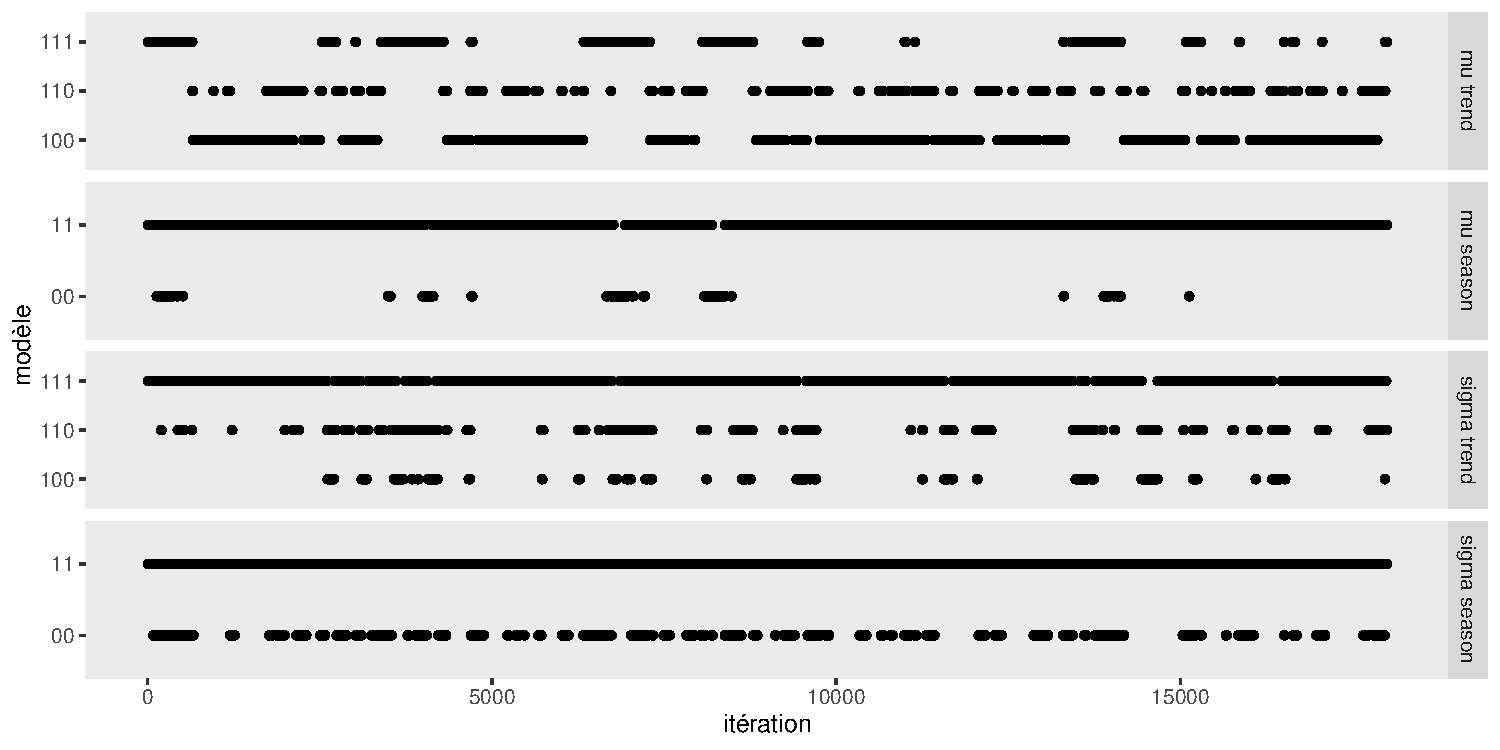
\includegraphics[width=\textwidth, center]{../figures/jumps.pdf}
	\end{figure}
\end{frame}


\begin{frame}{Modèles visités}
\begin{columns}
	\begin{column}{0.4\textwidth}
		\begin{figure}
		\vspace{-0.4cm}
	 		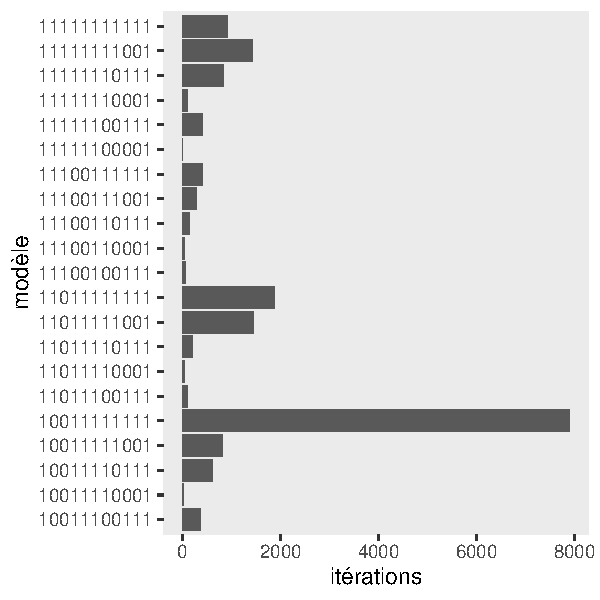
\includegraphics[height=0.85\textheight, center]{../figures/models.pdf}
		\end{figure}
	\end{column}
	\begin{column}{0.6\textwidth}
    Le modèle paramétrisé
    \begin{fleqn}
    \begin{equation*}
		\mu_t = \mu_0 + \mu_3 \cos(s_t) + \mu_4 \sin(s_t),
	\end{equation*}
	\begin{equation*}
		\sigma_t = \exp(\phi_0 + \phi_1 t + \phi_2 t^2 + \phi_3 \cos(s_t) + \phi_4 \sin(s_t)),
	\end{equation*}
	\begin{equation*}
		\xi_t = \xi,
	\end{equation*}
	\end{fleqn}
	est le plus visité.
	\vspace{0.5cm} \\
	Tous les modèles possibles ne sont pas visités pendant les 18000 itérations.
	\end{column}
\end{columns}
\end{frame}


\begin{frame}{Graphiques de trace}
\begin{columns}
	\begin{column}{0.65\textwidth}
		\begin{figure}
		\vspace{-0.4cm}
	 		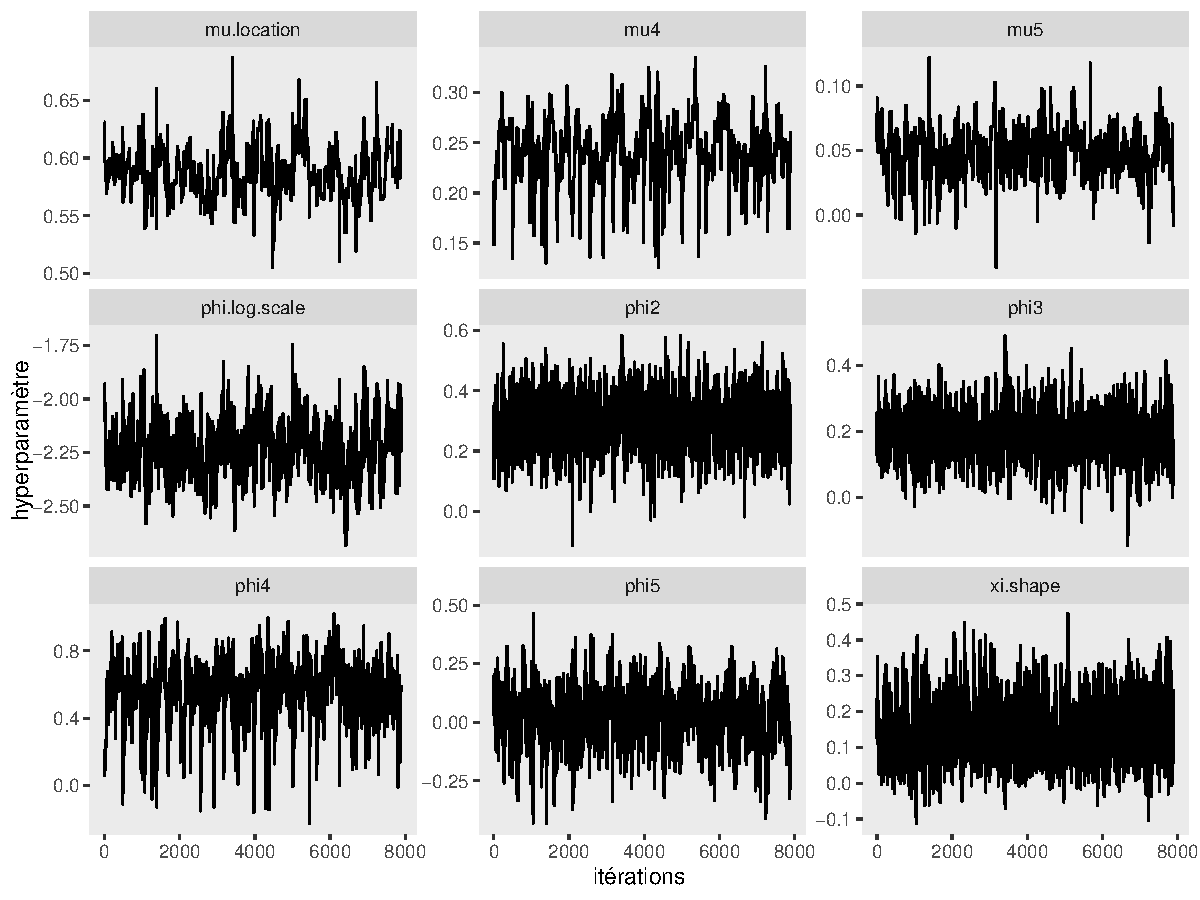
\includegraphics[height=0.9\textheight, center]{../figures/traces.pdf}
		\end{figure}
	\end{column}
	\begin{column}{0.35\textwidth}
    	\begin{itemize}
	\setlength{\itemsep}{10pt}
	\item Pseudo traces pour les 9 hyperparamètres du modèle le plus visité.
	\item Mixing des chaines $\mu$ moins bon que pour les autres paramètres.
	\item Période initiale de burn-in avant que les chaines soient stationnaires.
	\end{itemize}
	\end{column}
\end{columns}
\end{frame}


\begin{frame}{Distributions des hyperparamètres}
\begin{columns}
	\begin{column}{0.65\textwidth}
		\begin{figure}
		\vspace{-0.4cm}
	 		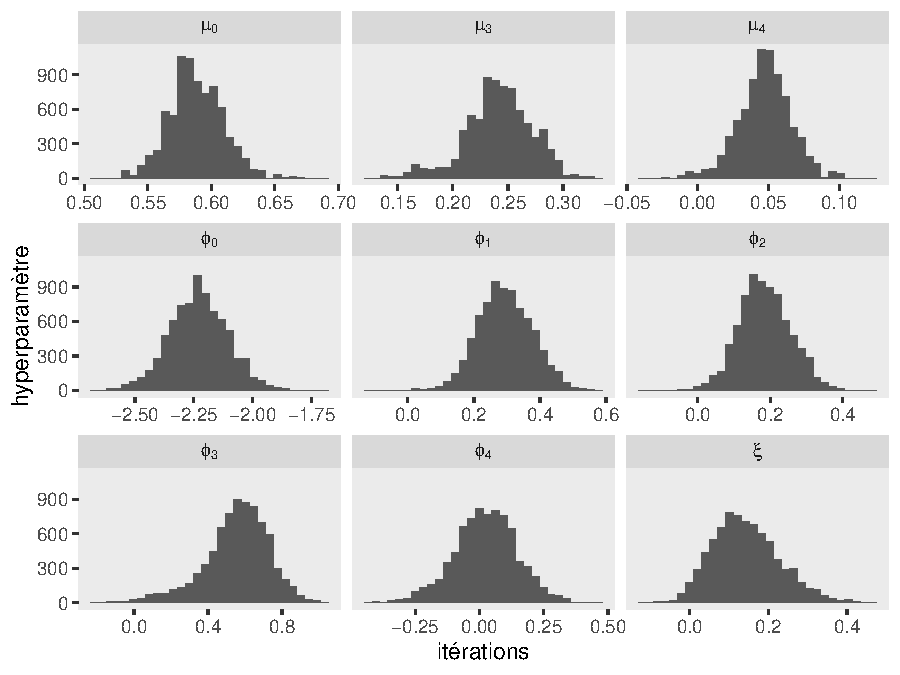
\includegraphics[height=0.9\textheight, center]{../figures/hists.pdf}
		\end{figure}
	\end{column}
	\begin{column}{0.35\textwidth}
	\begin{itemize}
	\setlength{\itemsep}{17pt}
	\item Hyperparamètres du modèle le plus visité.
	\item Des intervalles de crédibilité s'obtiennent avec le résultat du MCMC.
	\item Utilisable pour inférences avec incertitudes.
	\end{itemize}
	\end{column}
\end{columns}
\end{frame}


\begin{frame}{Conclusion}
\begin{itemize}
	\setlength{\itemsep}{17pt}
	\item L'approche POT permet une meilleure utilisation des données journalière que l'approche avec bloc maxima annuels,
	\item et permet de prendre en compte la saisonnalité.
	\item Un algorithme RJMCMC permet de facilement sélectionner un modèle parmi plusieurs,
	\item une bonne prise en compte des incertitudes,
	\item facilement adaptable à d'autres problèmes.
\end{itemize}
\end{frame}


%\section{Site d\rq{}étude et données}
%
%\subsection{Localisation des bassins versants dans l\rq{}aire urbaine d\rq{}Austin}
%
%\begin{frame}
%\begin{columns}
%	\begin{column}{0.75\textwidth}
%		\begin{figure}
%	 		\includegraphics[height=0.95\textheight, center]{intro_map.png}
%		\end{figure}
%	\end{column}
%	\begin{column}{0.25\textwidth}
%             	Zoom avec \emph{overview}.\\
%		\vspace{1cm}
%		{\scriptsize
%		\cite{united_states_census_bureau_census_2020, united_states_census_bureau_us_2021}}
%	\end{column}
%\end{columns}
%\end{frame}
%
%\subsection{Données d\rq{}occupation des sols}
%
%\begin{frame}
%\begin{columns}
%	\begin{column}{0.5\textwidth}
%		\begin{itemize}
%		\setlength{\itemsep}{10pt}
%		\item LU fournies pour 1990, 1995, 2000 et 2003.
%		\item Autres données disponibles pour 2010 et une date non-spécifiée.
%		\item Polygones avec classe de LU.
%		\item Données partiellement ou totalement inutilisables.
%		\end{itemize}
%	\end{column}
%	\begin{column}{0.5\textwidth}
%		\begin{itemize}
%		\setlength{\itemsep}{10pt}
%		\item Extraction des parcelles dans les BVs.
%		\item Recalcul de l\rq{}aire des parcelles.
%		\item Jointure de toutes les données de LU aux parcelles de 2010.
%		\item Polygones des routes absents en 2010 : calcul de la différence avec le  BV et fusion avec les autres parcelles.
%		\end{itemize}
%	\end{column}
%\end{columns}
%	\vspace{1cm}
%	{\scriptsize
%	\cite{city_of_austin_planning_and_development_review_2010_2021, city_of_austin_planning_and_development_review_land_2021}}
%\end{frame}
%
%\subsection{Données de topographie}
%
%\begin{frame}
%	\begin{figure}
%	 	\includegraphics[width=1.1\textwidth, center]{MNT_correction.png}
%	\end{figure}
%Décalage estimé par outils de mesure, puis correction des coordonnées ($‐50$ m en X et $+200$ m en Y).
%\end{frame}
%
%
%\section{Occupation des sols et urbanisation}
%
%\subsection{Méthode d\rq{}analyse de l\rq{}évolution de l\rq{}urbanisation}
%
%\begin{frame}{Classes d\rq{}occupation des sols}
%\begin{table}[ht]
%\centering
%\scriptsize
%\begin{tabularx}{\textwidth}{lllll}
%  \toprule
%indice urbanisation & classe simple & nom classe & classe complète & définition \\ 
%  \midrule
%  0 &   7 & espace verts & 700 & ? \\ 
%     &    &  & 710 & Parks/Greenbelts  \\ 
%     &    &  & 720 & Golf Courses  \\ 
%\vdots &  \vdots & \vdots & \vdots & \vdots \\
%     &   9 & agricole ou naturel & 910 & Agricultural \\ 
%     &    &  & 940 & Water  \\ 
%     &    &  & 999 & Unknown \\ 
%     \midrule
%\vdots &  \vdots & \vdots & \vdots & \vdots \\
%     \midrule
%    3 &   5 & industrie & 500 & ? \\ 
%\vdots &  \vdots & \vdots & \vdots & \vdots \\
%     &   8 & route ou transport & 800 & ? \\ 
%\vdots &  \vdots & \vdots & \vdots & \vdots \\
%   \bottomrule
%\end{tabularx}
%\end{table}
%\end{frame}
%
%\begin{frame}{Indice d\rq{}urbanisation}
%\begin{columns}
%	\begin{column}{0.5\textwidth}
%	\begin{block}{Calcul de champ}
%	CASE\\
%	WHEN LU1990 in (7, 9) THEN 0\\
%	WHEN LU1990 in (0, 1, 3) THEN 1\\
%	WHEN LU1990 in (2, 4, 6) THEN 2\\
%	WHEN LU1990 in (5, 8) THEN 3\\
%	END
%	\end{block}
%	\end{column}
%	\begin{column}{0.5\textwidth}
%		\begin{itemize}
%		\setlength{\itemsep}{10pt}
%		\item \lq\lq{}potentiel de ruissellement\rq\rq{} de la classe de LU.
%		\item Indice ordonné.
%		\item Permet de calculer une évolution.
%		\end{itemize}
%	\end{column}
%\end{columns}
%\end{frame}
%
%\subsection{Évolution de l\rq{}occupation des sols de 1990 à 2010}
%
%\begin{frame}
%\begin{columns}
%	\begin{column}{0.75\textwidth}
%	\begin{figure}
%	 	\includegraphics[height=0.97\textheight, center]{LandUse_Bull.png}
%	\end{figure}
%	\end{column}
%	\begin{column}{0.25\textwidth}
%	\begin{figure}
%	 	\begin{itemize}
%		\item Résultats présentés uniquement pour le BV de Bull.
%		\item Pas de routes en 1990 ?
%		\item Encore plus de problèmes pour le BV de Williamson.
%		\end{itemize}
%	\end{figure}
%	\end{column}
%\end{columns}
%\end{frame}
%
%\begin{frame}{Évolution de l\rq{}occupation pour le BV de Bull}
%\begin{columns}
%	\begin{column}{0.77\textwidth}
%		 \includegraphics[height=0.8\textheight, center]{LUbull_area.pdf}
%	\end{column}
%	\begin{column}{0.23\textwidth}
%		 \begin{itemize}
%		\item Diminution classe 9.
%		\item Augmentation classes 7 et 1.
%		\item Stabilité classe 8.
%		\item Disparition de la classe 0 en 2003, impact ?
%		\end{itemize}
%	\end{column}
%\end{columns}
%\end{frame}
%
%\begin{frame}{Évolution de l\rq{}indice d\rq{}urbanisation pour le BV de Bull}
%\includegraphics[width=1.13\textwidth ,center]{DeltaUrb.png}
%\end{frame}
%
%
%\section{Relation entre topographie, pente et occupation des sols}
%
%\subsection{Méthodes d\rq{}analyse des données topographiques}
%
%\begin{frame}{Création d\rq{}une couche avec LU, élévation et pente}
%	\begin{enumerate}
%	\setlength{\itemsep}{10pt}
%	\item Raster de pente créé à partir du MNT avec la fonction \emph{slope}.
%	\item Rasters de MNT et pente convertis en points.
%	\item Extraction des données de LU avec les points de MNT.
%	\item Jointure des points de LU, MNT et pente.
%	\item Couche exportable pour analyse dans R.
%	\end{enumerate}
%\end{frame}
%
%\subsection{Impact de la topographie sur l\rq{}occupation des sols et l\rq{}urbanisation}
%
%\begin{frame}{Topographie et pente du BV de Bull}
%\includegraphics[width=\textwidth, center]{topo_Bull.png}
%\end{frame}
%
%\begin{frame}{Lien \emph{local} entre relief et LU}
%\includegraphics[width=0.93\textwidth, center]{habitat_MNT.png}
%\end{frame}
%
%\begin{frame}{Topographie et pente du BV de Williamson et courbe hypsométrique}
%\begin{columns}
%	\begin{column}{0.65\textwidth}
%	\includegraphics[height=0.87\textheight, center]{topo_Williamson.png}
%	\end{column}
%	\begin{column}{0.35\textwidth}
%	\includegraphics[height=0.5\textheight, center]{courbe_hypso.pdf}
%	\end{column}
%\end{columns}
%\end{frame}
%
%\begin{frame}{Lien entre élévation et LU}
%\includegraphics[width=0.95\textwidth, center]{boxplot_MNT.pdf}
%\end{frame}
%
%\begin{frame}{Lien entre pente et LU}
%\includegraphics[width=0.95\textwidth, center]{boxplot_slope.pdf}
%\end{frame}
%
%\begin{frame}{Lien entre relief et la classe 5 \lq\lq{}industrie\rq\rq{}}
%\includegraphics[width=1.13\textwidth, center]{indus_slope.png}
%\end{frame}
%
%
%\section{Conclusion}
%
%\begin{frame}<beamer>{Plan}
%\frametitle{Plan}
%\tableofcontents[currentsection]
%\end{frame}
%
%\begin{frame}
% 	\begin{itemize}
% 	\setlength{\itemsep}{10pt}
%	\item Augmentation du degré d\rq{}urbanisation des BVs ...
%	\item ... principalement le long des routes majeures.
%	\item Pas de lien entre LU et altitude.
%	\item Quelques relations entre LU et pente.
%	\item Le réseau de transport semble plus déterminant que le relief ...
%	\item ... mais ce réseau pourrait aussi être dépendant du relief.
%	\item Plus de données devraient être analysées pour réellement conclure.
%	\end{itemize}
%\end{frame}

\section*{}

\begin{frame}[plain]{Références}
\printbibliography
\end{frame}

{
\setbeamercolor{background canvas}{bg=my_blue}
\begin{frame}[plain]
\begin{tikzpicture}[overlay, remember picture]
\node[anchor=center] at (current page.center) {
\begin{beamercolorbox}[center]{title}
     \centerline{\huge{\textcolor{white}{merci pour votre attention}}}
  \end{beamercolorbox}};
\end{tikzpicture}
\end{frame}
}


\end{document}


